
\documentclass[14pt]{extreport}
\usepackage{gost}
\usepackage{hyperref}
\usepackage{makecell}
\usepackage{ragged2e}
\justifying

\makeatletter
\@addtoreset{figure}{part}
\makeatother
\renewcommand{\thefigure}{\arabic{figure}}
\renewcommand{\thetable}{\arabic{table}}




\begin{document}
\pagestyle{empty} 
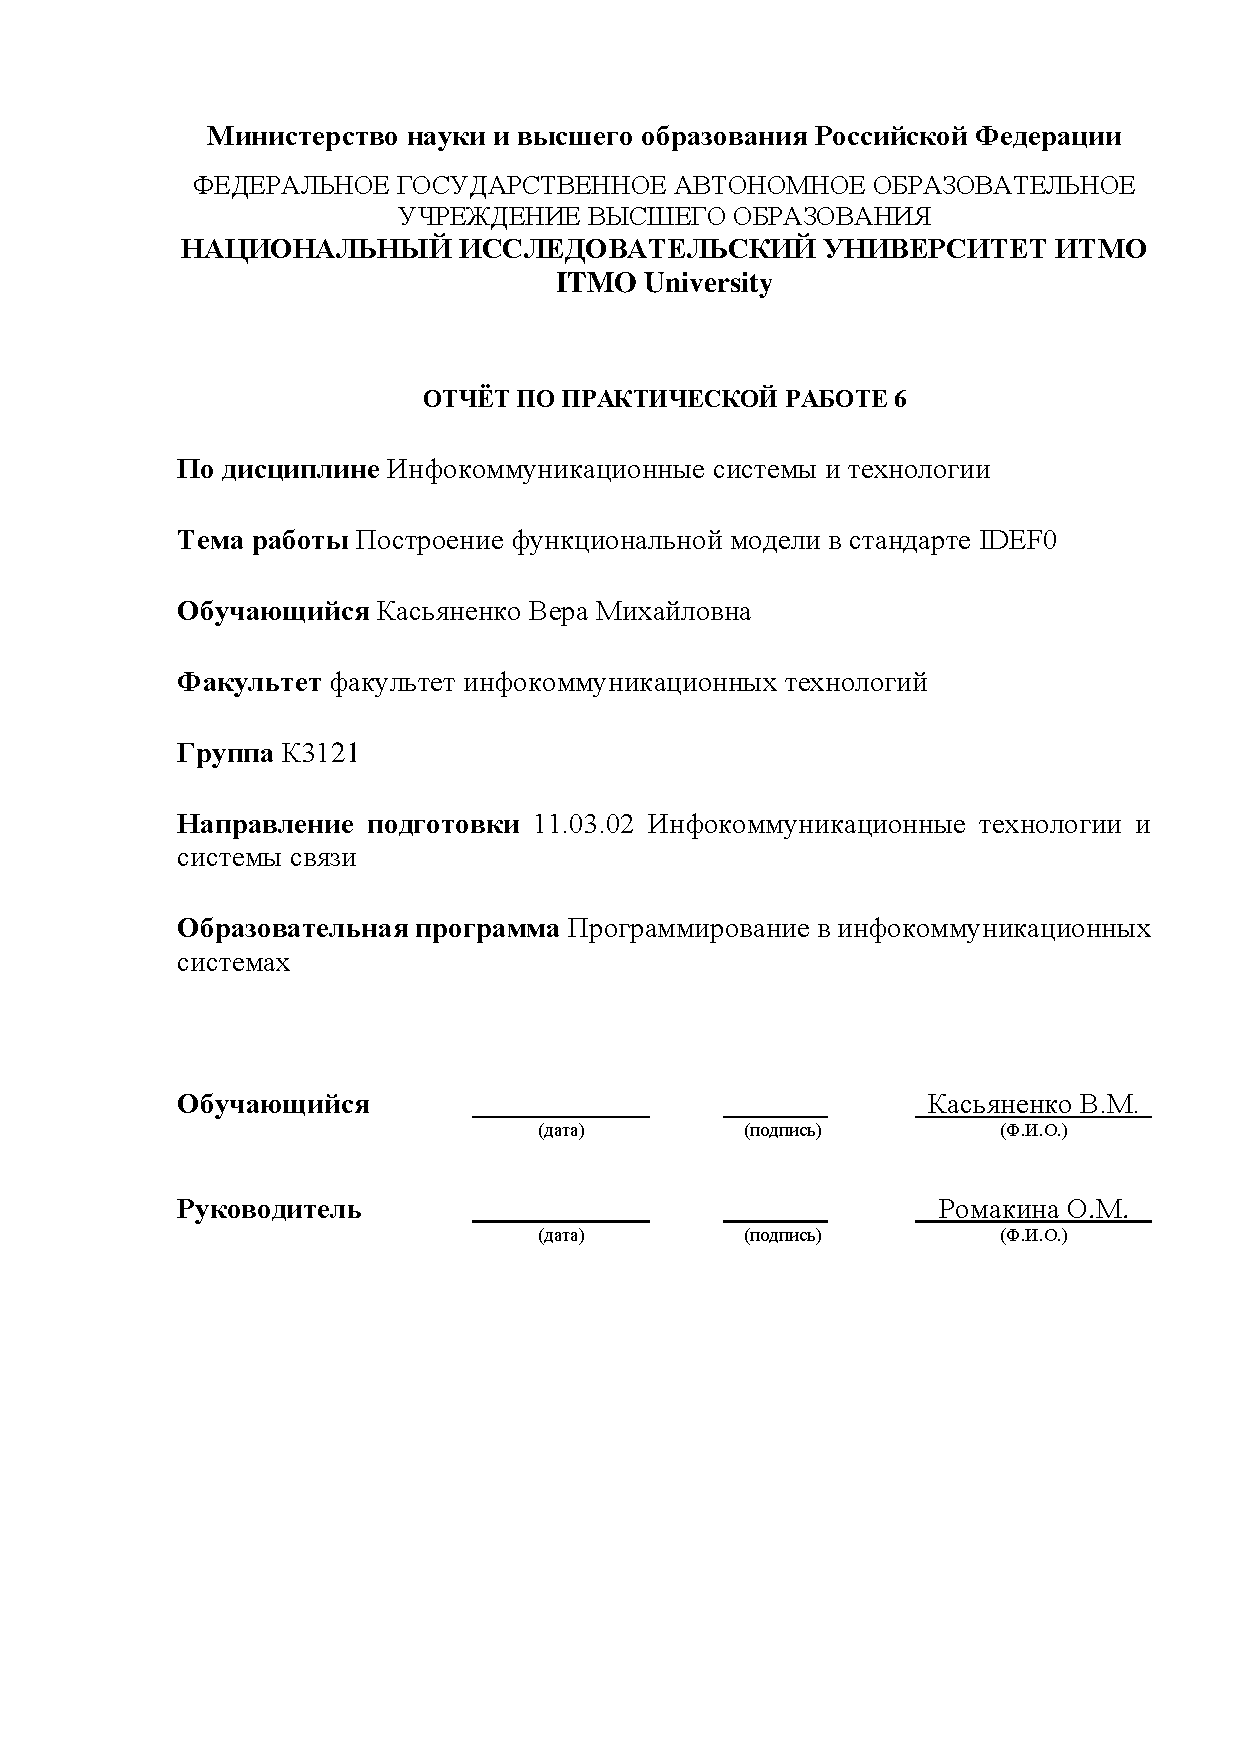
\includepdf[pages=-,pagecommand={}]{titulCourse.pdf}

\pagestyle{plain}
\tableofcontents
 



\intro 

В данном отчете будут представлены функциональные модели в стандарте IDEF0 для мобильного приложения OptiTune с точки зрения пользователя.


\chapter{Модели IDEF0\label{chapter1}}
\section{Функциональные модели в стандарте IDEF0}

В данном разделе представлены функциональные модели в стандарте IDEF0 с точки зрения пользователя приложения. Они представлены в виде контекстной диаграммы (рисунок \ref{fig1}) и декомпозиции этой диаграммы  (рисунок \ref{fig2}). Также для декомпозиции контекстной диаграммы представлены декомпозиции блоков "Определение уровня доступа в систему"\ (рисунок \ref{fig3}) и "Обработка запроса пользователя"\ (рисунок \ref{fig5}). Более того, для блока "Определение уровня доступа в систему" представлена декомпозиции блока "Авторизация"\ (рисунок \ref{fig4}).

\begin{landscape}
\begin{figure}[H]
\centerline{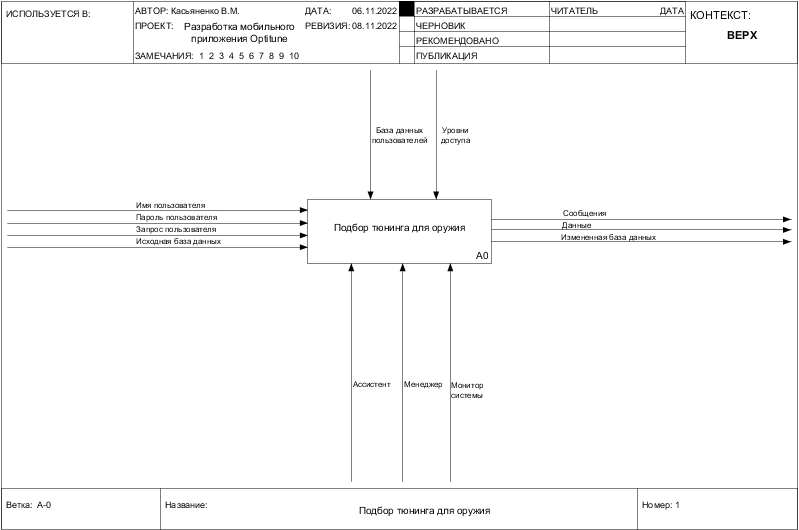
\includegraphics[width=0.9\linewidth]{01_A-0}}
\caption{Контекстная диаграмма}
\label{fig1}
\end{figure}

\begin{figure}[H]
\centerline{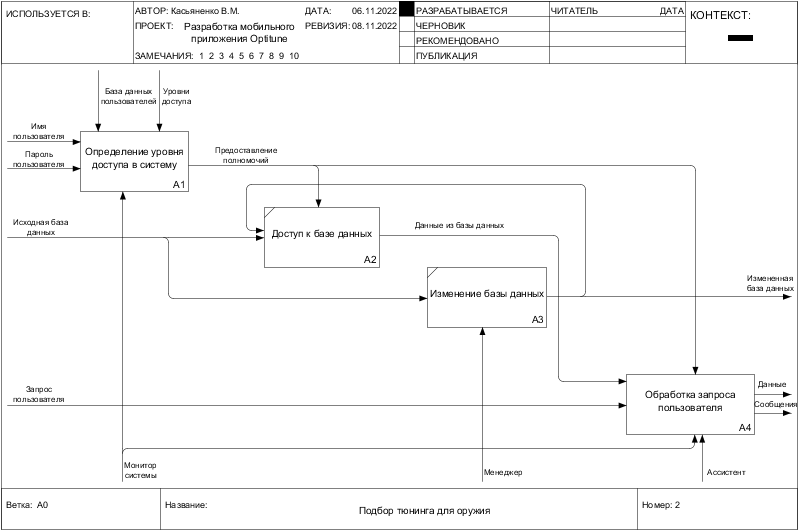
\includegraphics[width=0.9\linewidth]{02_A0}}
\caption{Декомпозиция контекстной диаграммы}
\label{fig2}
\end{figure}

\begin{figure}[H]
\centerline{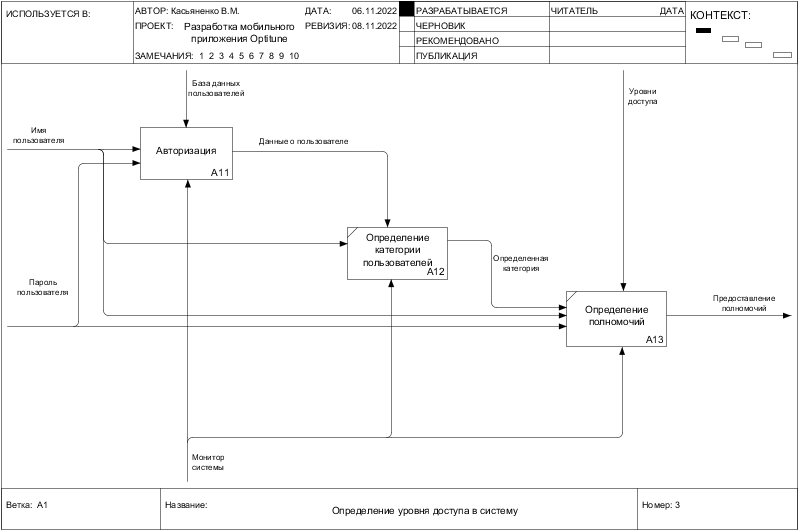
\includegraphics[width=0.9\linewidth]{03_A1}}
\caption{Декомпозиция блока "Определение уровня доступа в систему"}
\label{fig3}
\end{figure}

\begin{figure}[H]
\centerline{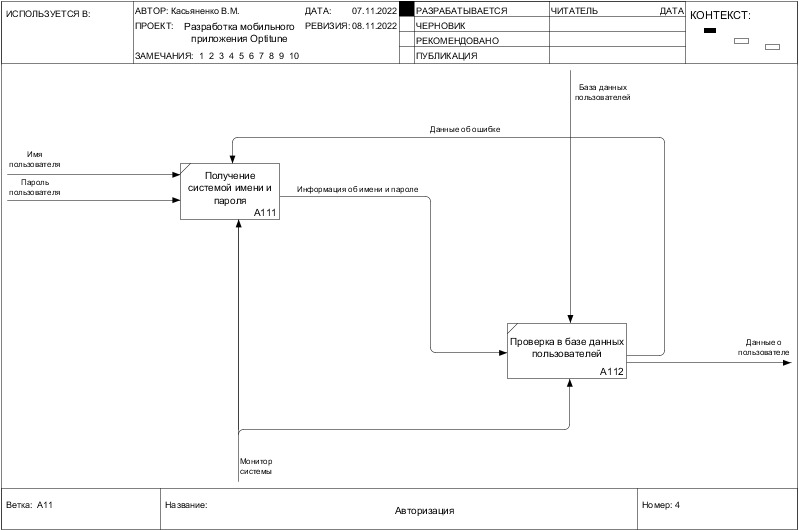
\includegraphics[width=0.9\linewidth]{04_A11}}
\caption{Декомпозиция блока "Авторизация"}
\label{fig4}
\end{figure}

\begin{figure}[H]
\centerline{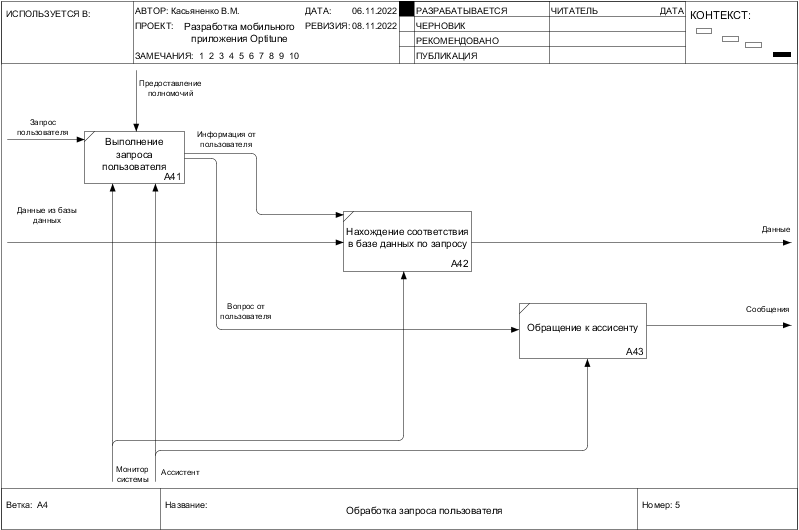
\includegraphics[width=0.9\linewidth]{05_A4}}
\caption{Декомпозиция блока "Обработка запроса пользователя"}
\label{fig5}
\end{figure}
\end{landscape}

\conclusions

Был составлен отчет, в котором были представлены функциональные модели IDEF0 с точки зрения пользователя мобильного приложения OptiTune.



\newpage
\begin{thebibliography}{99}

\bibitem{bib1} Wikipedia: официальный сайт. – URL: \url{https://ru.wikipedia.org/wiki/IDEF} (Дата обращения 07.11.2022).

\end{thebibliography}







\end{document}
